% Copyright 2004 by Till Tantau <tantau@users.sourceforge.net>.
%
% In principle, this file can be redistributed and/or modified under
% the terms of the GNU Public License, version 2.
%
% However, this file is supposed to be a template to be modified
% for your own needs. For this reason, if you use this file as a
% template and not specifically distribute it as part of a another
% package/program, I grant the extra permission to freely copy and
% modify this file as you see fit and even to delete this copyright
% notice. 

\documentclass{beamer}
% There are many different themes available for Beamer. A comprehensive
% list with examples is given here:
% http://deic.uab.es/~iblanes/beamer_gallery/index_by_theme.html
% You can uncomment the themes below if you would like to use a different
% one:
%\usetheme{AnnArbor}
%\usetheme{Antibes}
%\usetheme{Bergen}
%\usetheme{Berkeley}
%\usetheme{Berlin}
%\usetheme{Boadilla}
%\usetheme{boxes}
%\usetheme{CambridgeUS}
%\usetheme{Copenhagen}
%\usetheme{Darmstadt}
%\usetheme{default}
%\usetheme{Frankfurt}
%\usetheme{Goettingen}
%\usetheme{Hannover}
%\usetheme{Ilmenau}
%\usetheme{JuanLesPins}
%\usetheme{Luebeck}
\usetheme{Madrid}
%\usetheme{Malmoe}
%\usetheme{Marburg}
%\usetheme{Montpellier}
%\usetheme{PaloAlto}
%\usetheme{Pittsburgh}
%\usetheme{Rochester}
%\usetheme{Singapore}
%\usetheme{Szeged}
%\usetheme{Warsaw}
\graphicspath{{figures/}}
\definecolor{cwired}{rgb}{0.803,0.0,0.227}
\setbeamercolor{structure}{fg=cwired}
\title{Causal Dynamic Time Lag (CDT)}

% A subtitle is optional and this may be deleted
\subtitle{Applications to Space Weather}

\author{Mandar ~Chandorkar}
% - Give the names in the same order as the appear in the paper.
% - Use the \inst{?} command only if the authors have different
%   affiliation.

\institute[CWI \& INRIA] % (optional, but mostly needed)
{
  \inst{1}%
  Multiscale Dynamics\\
  CWI, Amsterdam
  \and
  \inst{2}%
  TAO Research Unit\\
  INRIA, CNRS, Saclay}
% - Use the \inst command only if there are several affiliations.
% - Keep it simple, no one is interested in your street address.

\date{12 June 2018}
% - Either use conference name or its abbreviation.
% - Not really informative to the audience, more for people (including
%   yourself) who are reading the slides online

\subject{Machine Learning}
% This is only inserted into the PDF information catalog. Can be left
% out. 

% If you have a file called "university-logo-filename.xxx", where xxx
% is a graphic format that can be processed by latex or pdflatex,
% resp., then you can add a logo as follows:

\pgfdeclareimage[height=0.5cm]{university-logo}{figures/inria-logo}
\logo{\pgfuseimage{university-logo}}

% Delete this, if you do not want the table of contents to pop up at
% the beginning of each subsection:
\AtBeginSubsection[]
{
  \begin{frame}<beamer>{Outline}
    \tableofcontents[currentsection,currentsubsection]
  \end{frame}
}

% Let's get started
\begin{document}

\begin{frame}
  \titlepage
\end{frame}

\begin{frame}{Outline}
  \tableofcontents
  % You might wish to add the option [pausesections]
\end{frame}

\section{Motivation}

\subsection{Space Weather}

\begin{frame}
\begin{figure}[h]
        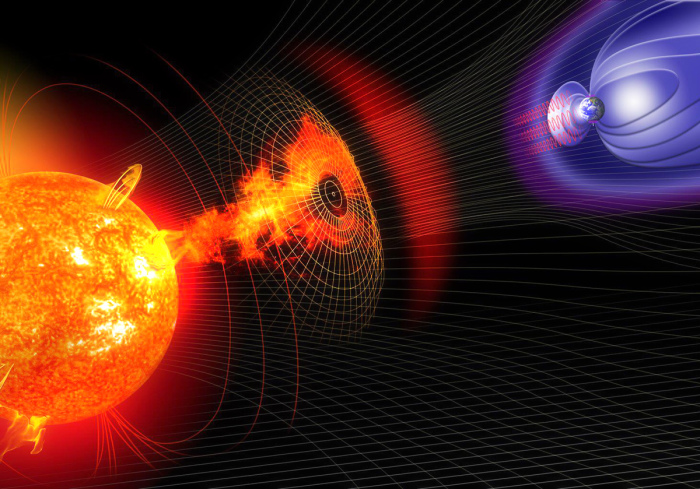
\includegraphics[width=0.85\textwidth]{space-weather.jpg}
        \caption{The Sun-Earth system}
        \label{fig:sun-earth}
\end{figure}
\end{frame}

\begin{frame}
\begin{figure}[h]
        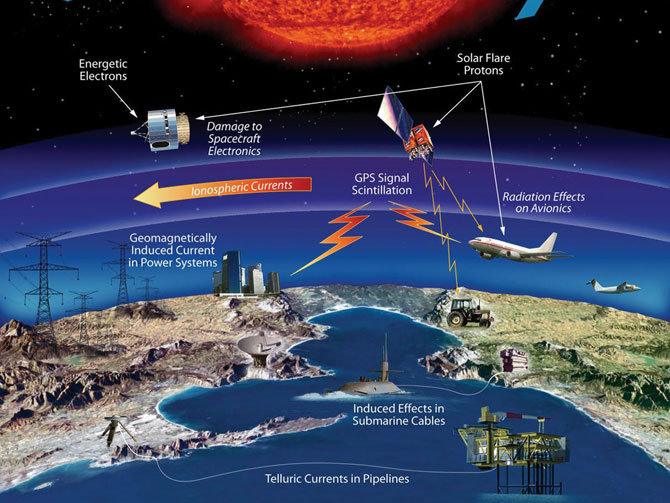
\includegraphics[width=0.85\textwidth]{nasa-space-weather.jpg}
        \caption{Effects of Solar Disturbances}
        \label{fig:sun-earth-nasa}
\end{figure}
\end{frame}

\subsection{Financial Markets}

\begin{frame}
\begin{figure}[h]
        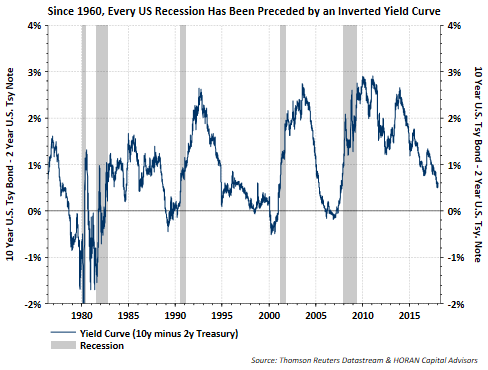
\includegraphics[width=0.80\textwidth]{spread-vs-stocks.png}
        \caption{Yield curves and Recessions in the U.S. Economy}
        \label{fig:fed-rate}
\end{figure}
\end{frame}

\section{Causality in Time Series}

\subsection{Concepts}

\begin{frame}{Granger Causality}
\begin{enumerate}
\item The cause happens prior to its effect.
\item The cause has unique information about the future values of its effect.
\end{enumerate}
\end{frame}

\begin{frame}
\begin{figure}[h]
        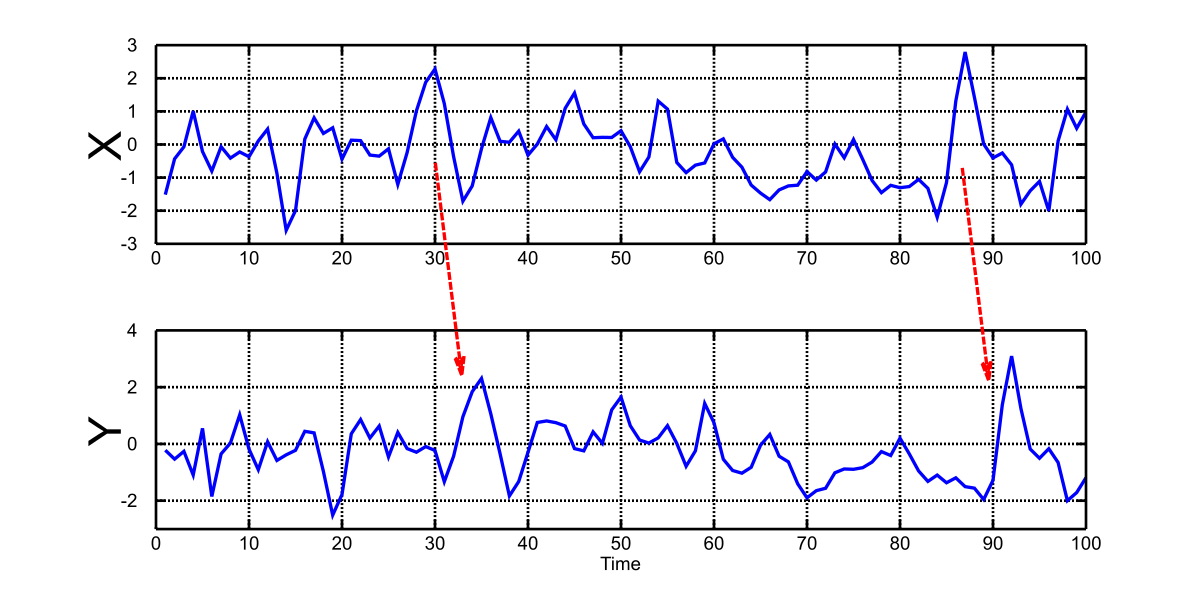
\includegraphics[width=0.80\textwidth]{GrangerCausality.png}
        \caption{By BiObserver - Own work, CC BY-SA 3.0, https://commons.wikimedia.org/w/index.php?curid=33470670}
        \label{fig:granger}
\end{figure}
\end{frame}

\subsection{Existing Research}

\begin{frame}{Nonparametric learning of time-lag}

\cite{ZHOU2006195} formulated the problem as minimisation of the \emph{mismatch} between two time series.

\textbf{Inputs}: $X(t), Y(t)$, two time series.

\textbf{Learn}: A mapping $\phi(t_1) = t_2$ which minimises 

\begin{equation}
\epsilon(t_t, t_2) = |X(t_1) - Y(t_2)|
\end{equation}


\end{frame}

\begin{frame}
\begin{figure}[h]
        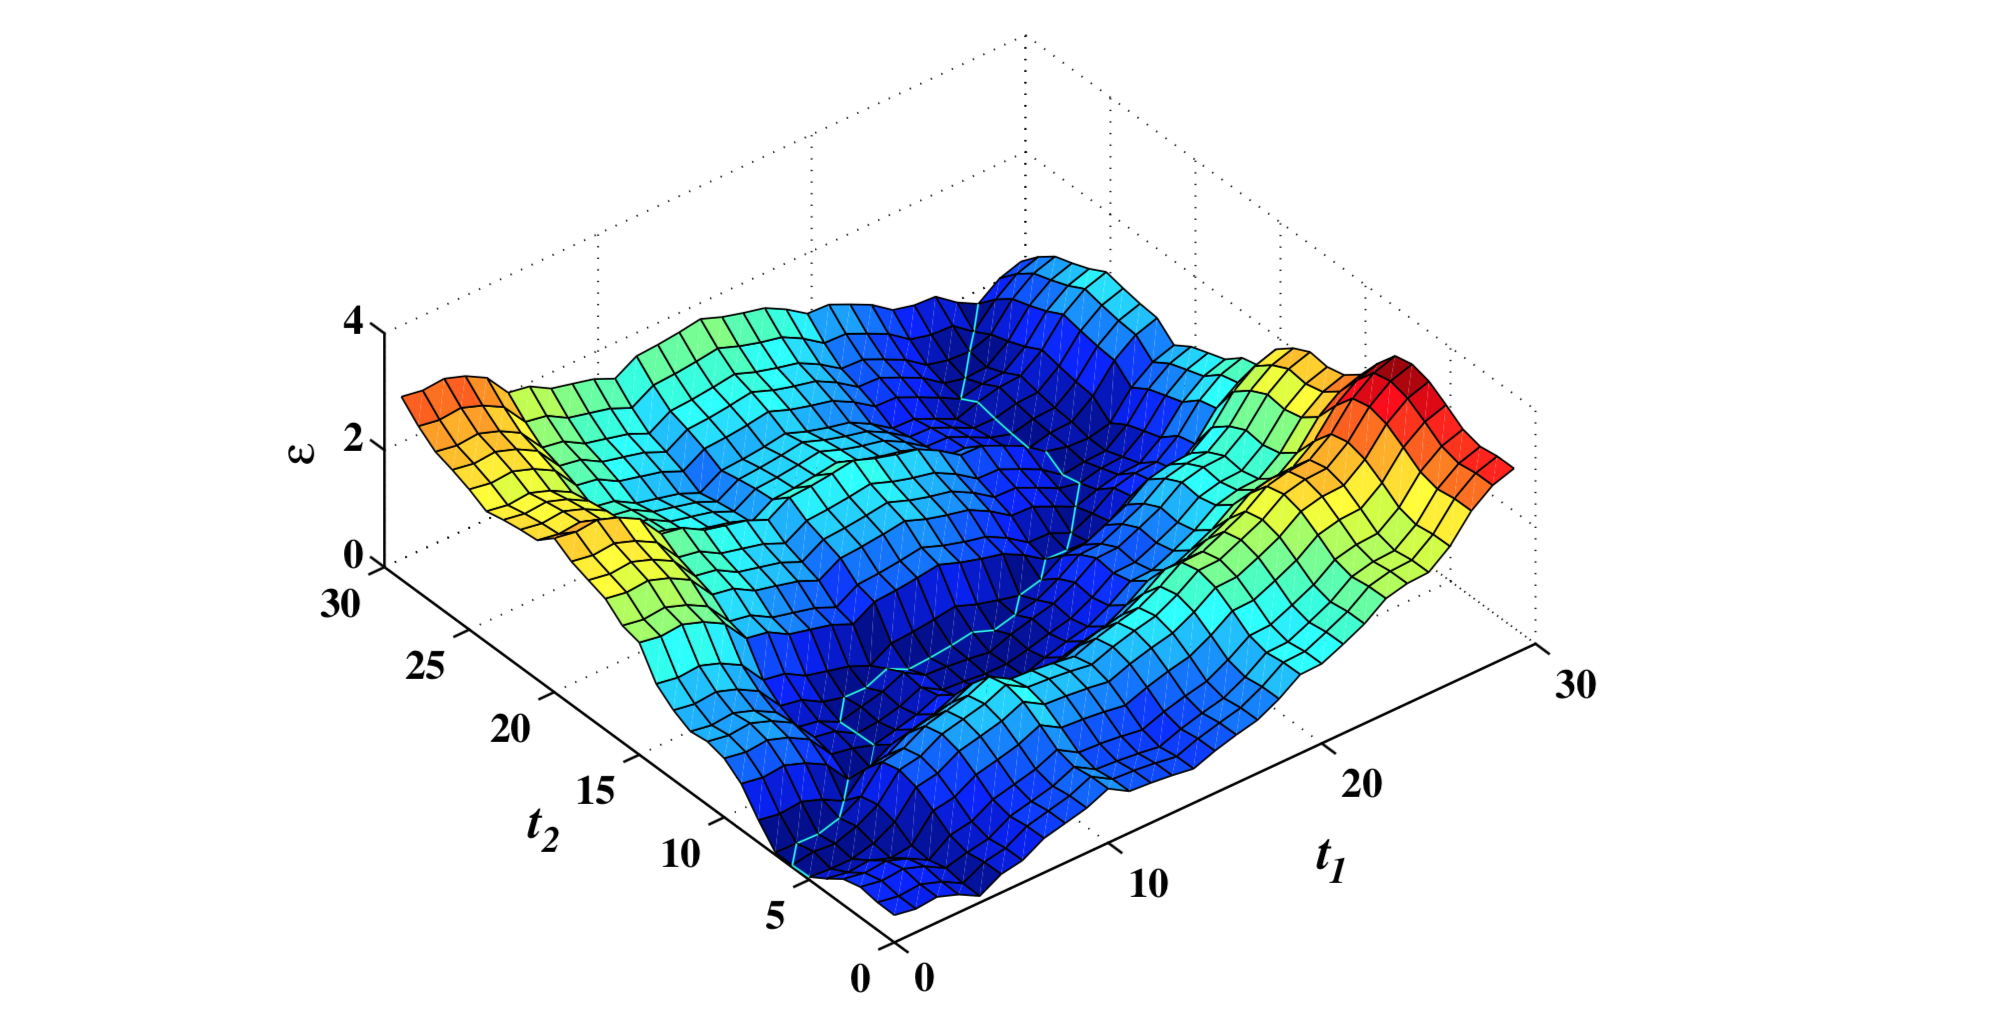
\includegraphics[width=0.90\textwidth]{polymer-alignment.png}
        \caption{An example of energy landscape $E_{X,Y}$ given by (1) for two noisy time series and the corresponding optimal path wandering at the bottom of the valley similarly to a river. This optimal path defines the mapping $t1 \rightarrow t2 = \phi(t1)$.}
        \label{fig:polymer}
\end{figure}
\end{frame}


% Section and subsections will appear in the presentation overview
% and table of contents.
\section{Problem \& Model}

\subsection{Description}

\begin{frame}{Causal Dynamic Time-lag Inference (CDT)}
  Given an input (cause) and output (effect) time series, predict 
  \begin{itemize}
  \item {
      Magnitude of output signal. (What/How much)
  }
  \item {
      When the effect will be observed in the output signal (When)
  }
  \end{itemize}
\end{frame}

\begin{frame}{CDT: Formal Definition}
\textbf{Input Signal} (Cause)

\begin{align*}
t &\in \mathbb{R}^+\\
x(t) &\in \mathcal{X}
\end{align*}

\textbf{Output Signal} (Effect)

\begin{align*}
f: \mathcal{X} &\rightarrow \mathbb{R}\\
g: \mathcal{X} &\rightarrow \mathbb{R}^+\\
\Delta(t) &= g[x(t)] \\
y(t + \Delta(t)) &= f[x(t)] 
\end{align*}

\end{frame}

\subsection{Proposed Solution}

\begin{frame}{Model Specification}

\textbf{Input Patterns} $x(t)$ \newline

\textbf{Causal Time Window} \newline
\textit{Lower Limit}: $\ell \in \mathbb{N} \cup 0$ \newline
\textit{Upper Limit}: $\ell + h: h \in \mathbb{N}$ \newline

\textbf{Targets} $y(t+\ell), \cdots, y(t+\ell+h-1)$ \newline

\textbf{Model Outputs} \newline
\textit{Predictions} $\hat{y}(t+\ell), \cdots, \hat{y}(t+\ell+h-1)$ \newline
\textit{Time Lag Probabilities} $\hat{p}(t+\ell), \cdots, \hat{p}(t+\ell+h-1)$
    
\end{frame}

\begin{frame}{Training: Motivation}
Balance two incentives

\begin{enumerate}
    \item Generate accurate predictions for time window $y(t+\ell), \cdots, y(t+\ell+h-1)$
    \newline
    \item Learn time lag structure according to some prior.
\end{enumerate}
\end{frame}

\begin{frame}{Training Loss}
\begin{align*}
\mathcal{L}(y^{(1:M)}, \hat{y}^{(1:M)}, \hat{p}^{(1:M)}) = &\lambda_1 \sum_{i,m}{\frac{1}{2M} (y^{(m)}_{i} - \hat{y}^{(m)}_{i})^2 (1 + \hat{p}^{(m)}_i)} \\ &+ \\ &\lambda_2 \mathcal{J}(y^{(1:M)}, \hat{y}^{(1:M)}, \hat{p}^{(1:M)})
\end{align*}
\end{frame}

\begin{frame}{Training Loss: Prior}
The term $\mathcal{J}(y^{(1:M)}, \hat{y}^{(1:M)}, \hat{p}^{(1:M)})$ penalizes the predicted probabilities $\hat{p}^{(1:M)}$, for deviation from some chosen \textit{target probability}.
    
\end{frame}

\begin{frame}{Prior: Target Probability}
The \textit{target probability} $\widetilde{p}$ for a time window $[t+\ell, t+\ell+h-1]$ can be characterized by:
\newline

\begin{block}{Conjecture: Causal Time Lag}
The lagged output $y(t+i)$ which has greater predictability given $x(t)$, is a more likely causal link. 
\end{block}

    
\end{frame}


\begin{frame}{Prior Contd.}

\begin{enumerate}
\item The target probability distribution for the time lag is, $\widetilde{p}^{(m)} = softmax( (y^{(m)} - \hat{y}^{(m)})^{2}/T )$
\newline
\item The term $\mathcal{J}(y^{(1:M)}, \hat{y}^{(1:M)}, \hat{p}^{(1:M)})$ can be computed as the \emph{Hellinger distance} between $\hat{p}$ and $\widetilde{p}$.
\end{enumerate}
\end{frame}

\begin{frame}
\begin{align*}
\mathcal{J}(y^{(1:M)}, \hat{y}^{(1:M)}, \hat{p}^{(1:M)}) &= \sum_{m = 1}^{M}{\frac{1}{M} \sqrt{\sum_{i}{(\sqrt{\widetilde{p}^{(m)}_i} -  \sqrt{\hat{p}^{(m)}_i})^2}}} \\\\
\widetilde{p}^{(m)} &= softmax( (y^{(m)} - \hat{y}^{(m)})^{2}/T )
\end{align*}
\end{frame}


\section{Applications}

\begin{frame}{Toy Problems}

\begin{align*}
 x(t+1) &= (1 - \beta) x(t) + \mathcal{N}(0, \sigma^2) \\
 y(t+\Delta(t)) &= \alpha ||x(t)||^2
\end{align*}

\begin{block}{Problem I: Constant Lag}
$\Delta(t) = k$
\end{block}

\begin{block}{Problem II: Constant Velocity $||x(t)||^2$; Fixed Distance $d$}
$\Delta(t) = d/(\alpha ||x(t)||^2)$
\end{block}

\begin{block}{Problem III: Constant Acceleration $a$; Fixed Distance $d$}
$\Delta(t) = (\sqrt{\alpha^2||x(t)||^4 - 2ad} - \alpha||x(t)||^2)/a$
\end{block}

\end{frame}

\subsection{Problem I}
\begin{frame}{Data}
    \begin{figure}[h]
        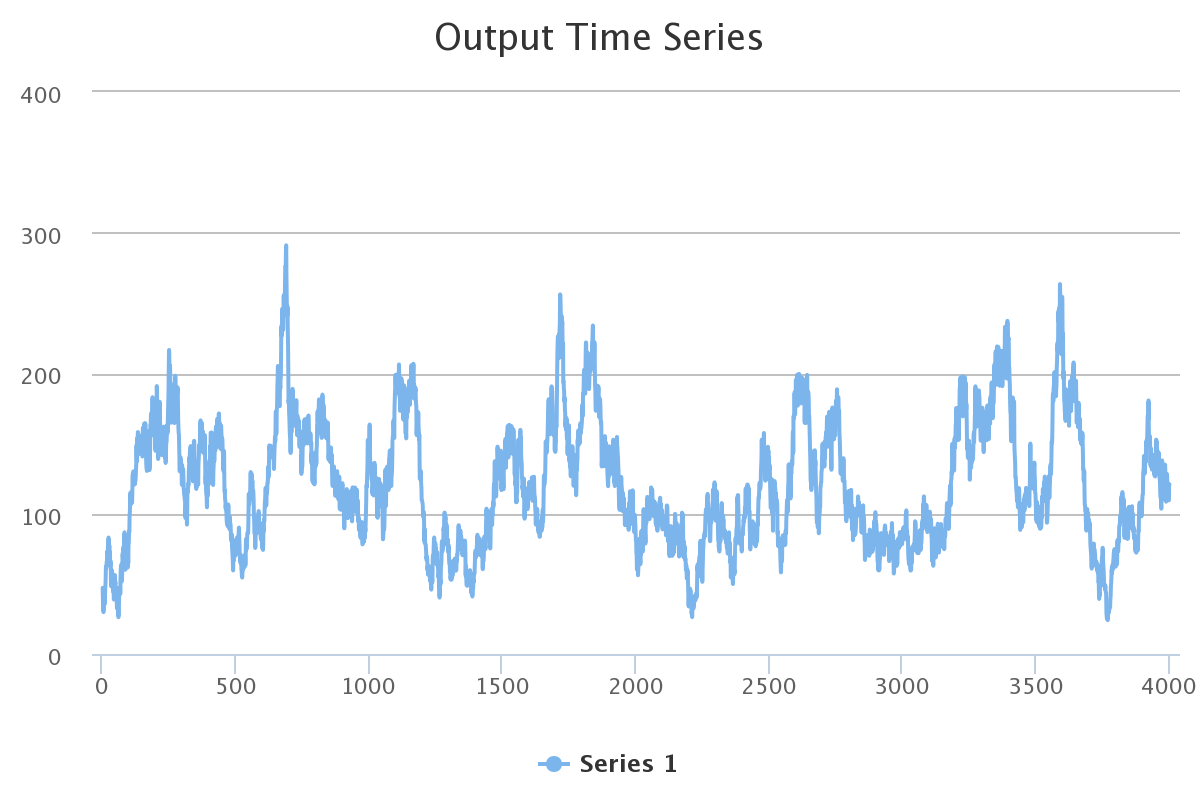
\includegraphics[width=0.75\textwidth]{timeseries-problem-i.png}
        \caption{Generated Data}
        \label{fig:TimeSeries-i}
      \end{figure}
\end{frame}


\begin{frame}{Predictions}
    \begin{figure}[h]
        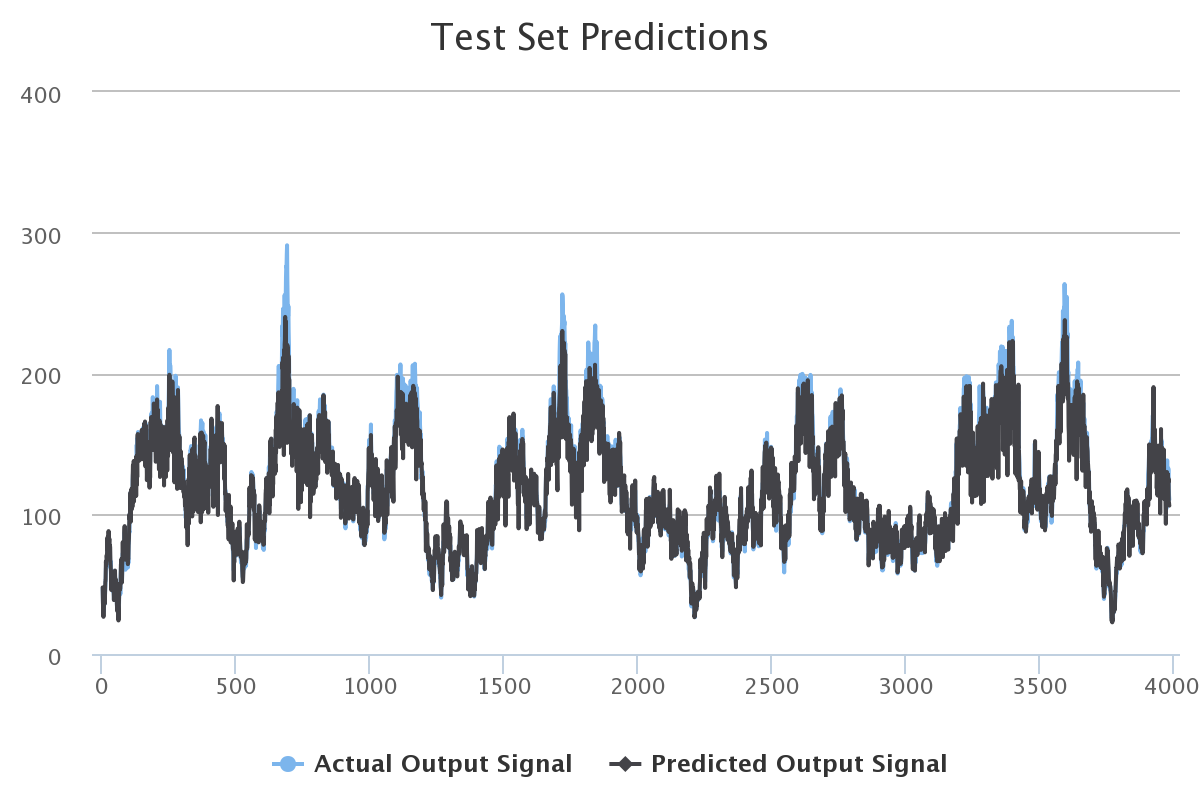
\includegraphics[width=0.75\textwidth]{predictions-i.png}
        \caption{Test Set Time Series vs Predictions}
        \label{fig:predictions-i}
      \end{figure}
\end{frame}

\begin{frame}{Errors}
    \begin{figure}[h]
        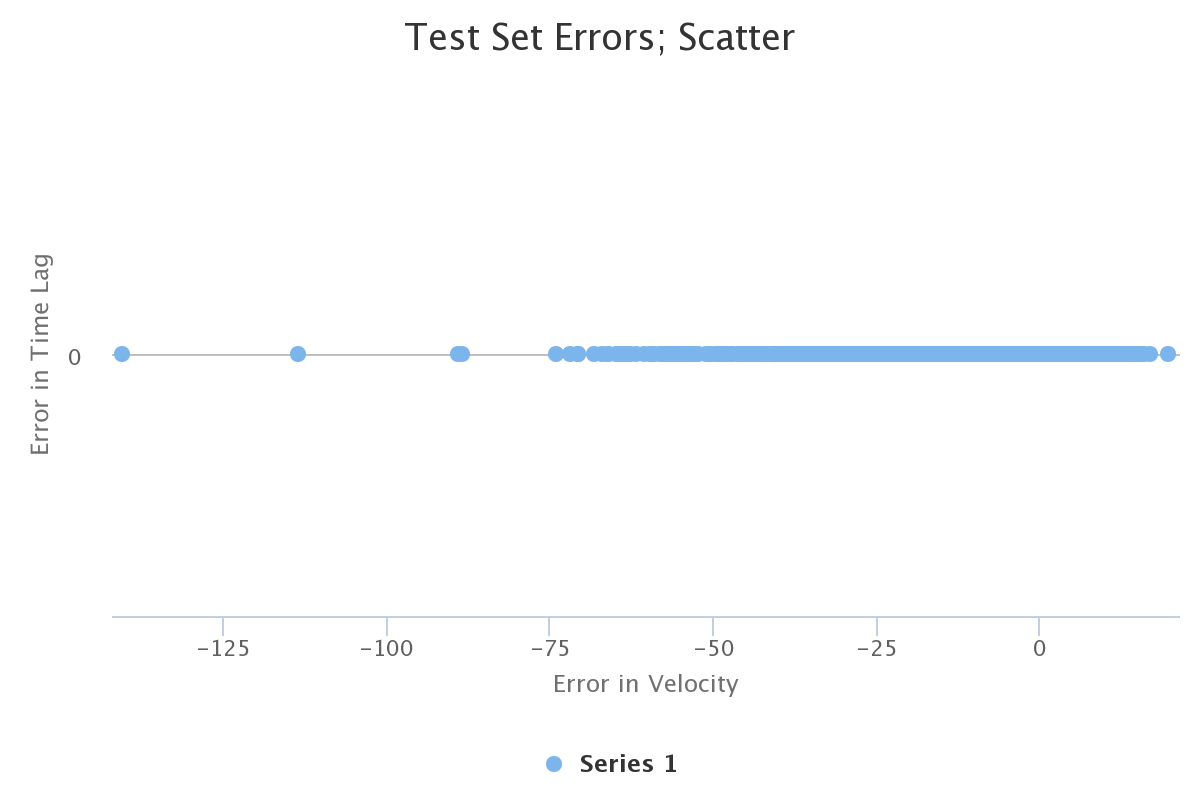
\includegraphics[width=0.75\textwidth]{errors-i.png}
        \caption{Error in Output vs Error in Time Lag}
        \label{fig:errors-i}
      \end{figure}
\end{frame}

\begin{frame}{Performance}
 
\begin{block}{Output}
\textbf{MAE}: 8.602 \\
\textbf{Pearson Corr}: 0.964 \\
\textbf{Spearman Corr}: 0.999
\end{block}

\begin{block}{Time Lag}
\textbf{MAE}: 0 \\
\textbf{Pearson Corr}: N.A \\
\textbf{Spearman Corr}: 1.0
\end{block}



\end{frame}



\subsection{Problem II}
\begin{frame}{Data}
    \begin{figure}[h]
        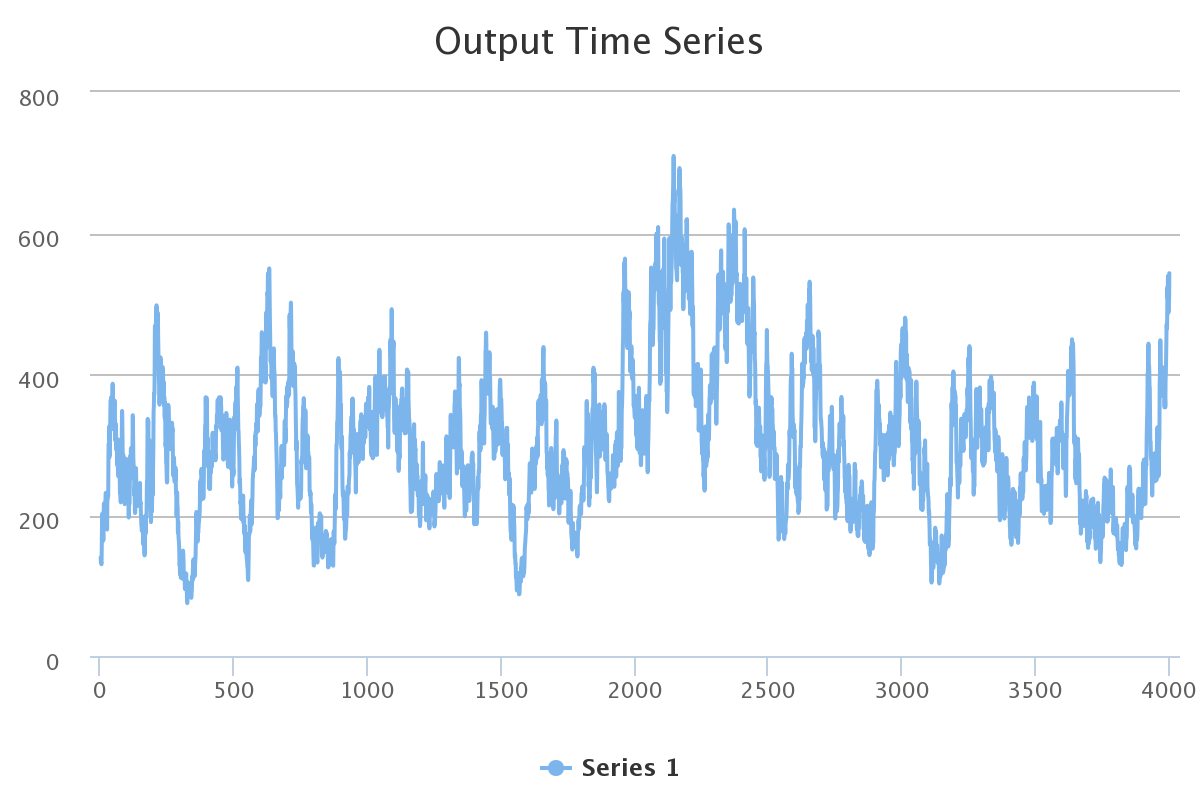
\includegraphics[width=0.75\textwidth]{timeseries-problem-ii.png}
        \caption{Generated Data}
        \label{fig:TimeSeries-ii}
      \end{figure}
\end{frame}

\begin{frame}{Time Lags}
    \begin{figure}[h]
        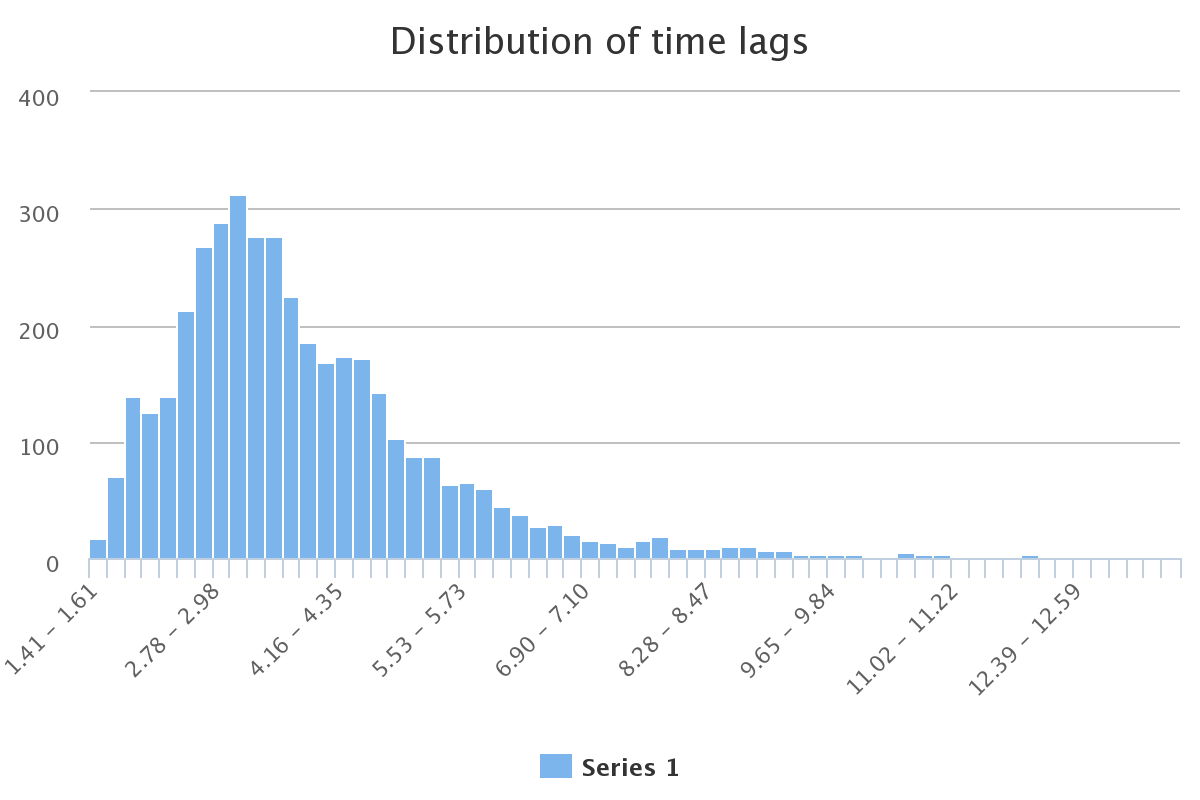
\includegraphics[width=0.75\textwidth]{data-hist-problem-ii.png}
        \caption{Time Lags}
        \label{fig:TimeLags-ii}
      \end{figure}
\end{frame}

\begin{frame}{Test Data Distribution}
    \begin{figure}[h]
        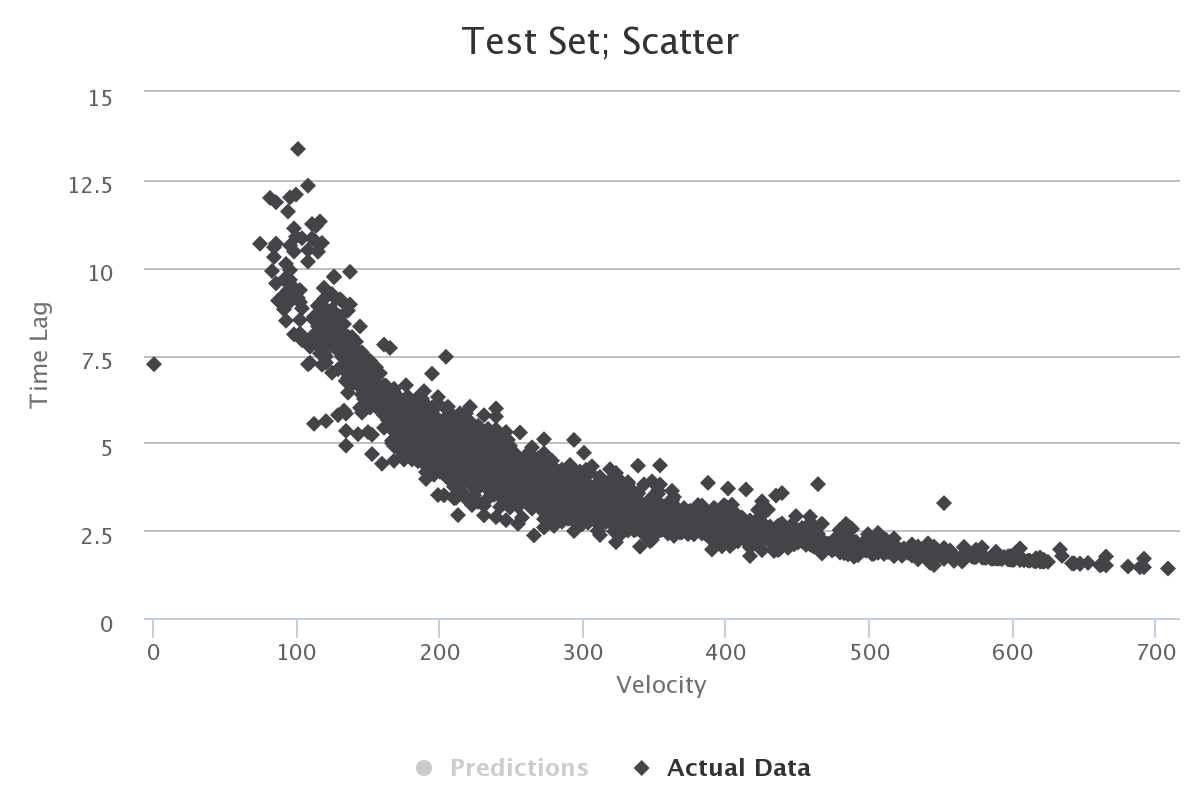
\includegraphics[width=0.75\textwidth]{data-scatter-ii.png}
        \caption{Output vs Time Lags}
        \label{fig:VelTimeLags-ii}
      \end{figure}
\end{frame}


\begin{frame}{Predictions}
    \begin{figure}[h]
        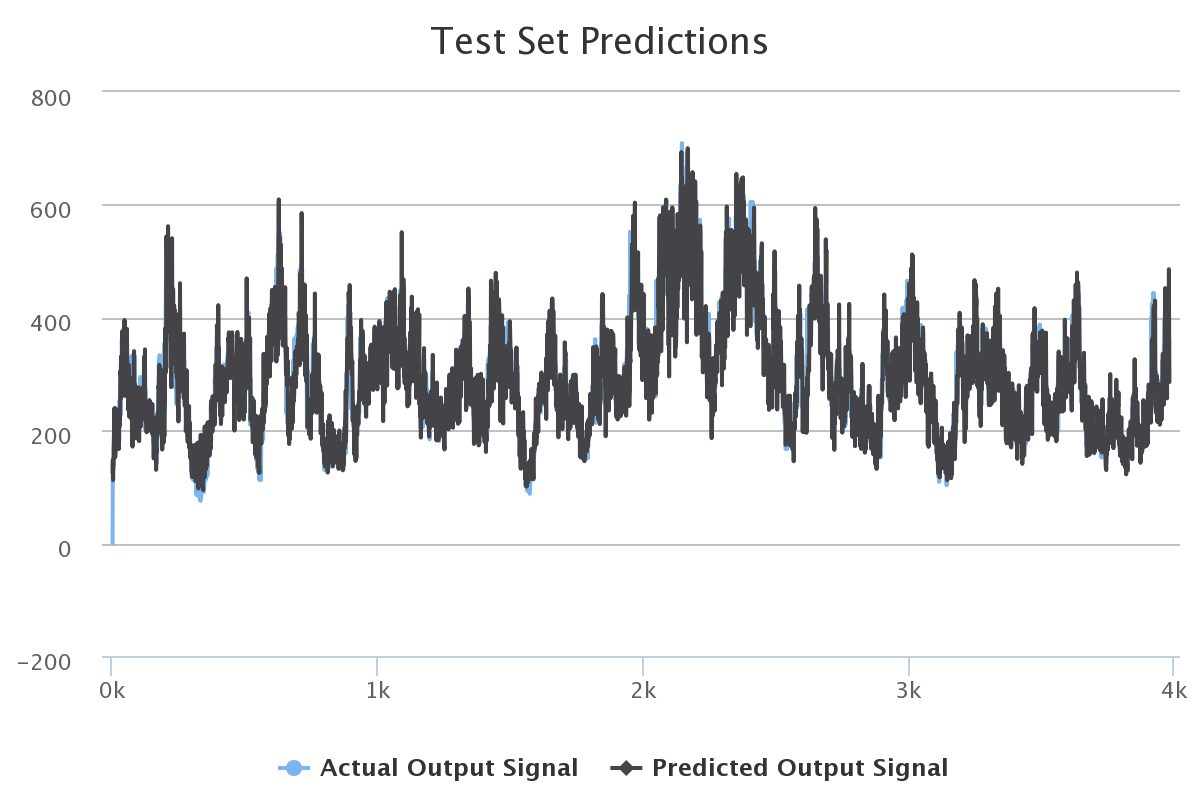
\includegraphics[width=0.75\textwidth]{predictions-ii.png}
        \caption{Test Set Time Series vs Predictions}
        \label{fig:predictions-ii}
      \end{figure}
\end{frame}

\begin{frame}{Errors}
    \begin{figure}[h]
        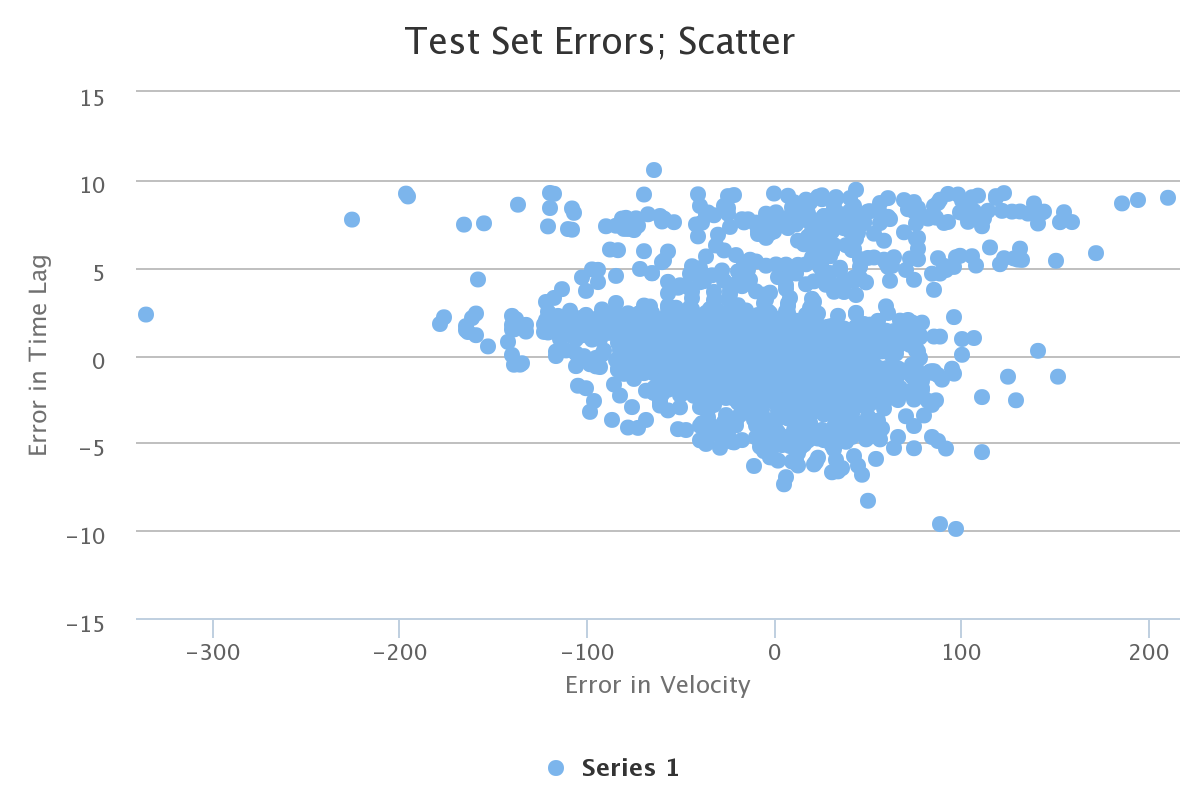
\includegraphics[width=0.75\textwidth]{errors-ii.png}
        \caption{Error in Output vs Error in Time Lag}
        \label{fig:errors-ii}
      \end{figure}
\end{frame}

\begin{frame}{Performance}
 
\begin{block}{Output}
\textbf{MAE}: 30.902 \\
\textbf{Pearson Corr}: 0.918 \\
\textbf{Spearman Corr}: 0.999
\end{block}

\begin{block}{Time Lag}
\textbf{MAE}: 1.593 \\
\textbf{Pearson Corr}: 0.337 \\
\textbf{Spearman Corr}: 0.999
\end{block}



\end{frame}

\subsection{Problem III}

\begin{frame}{Data}
    \begin{figure}[h]
        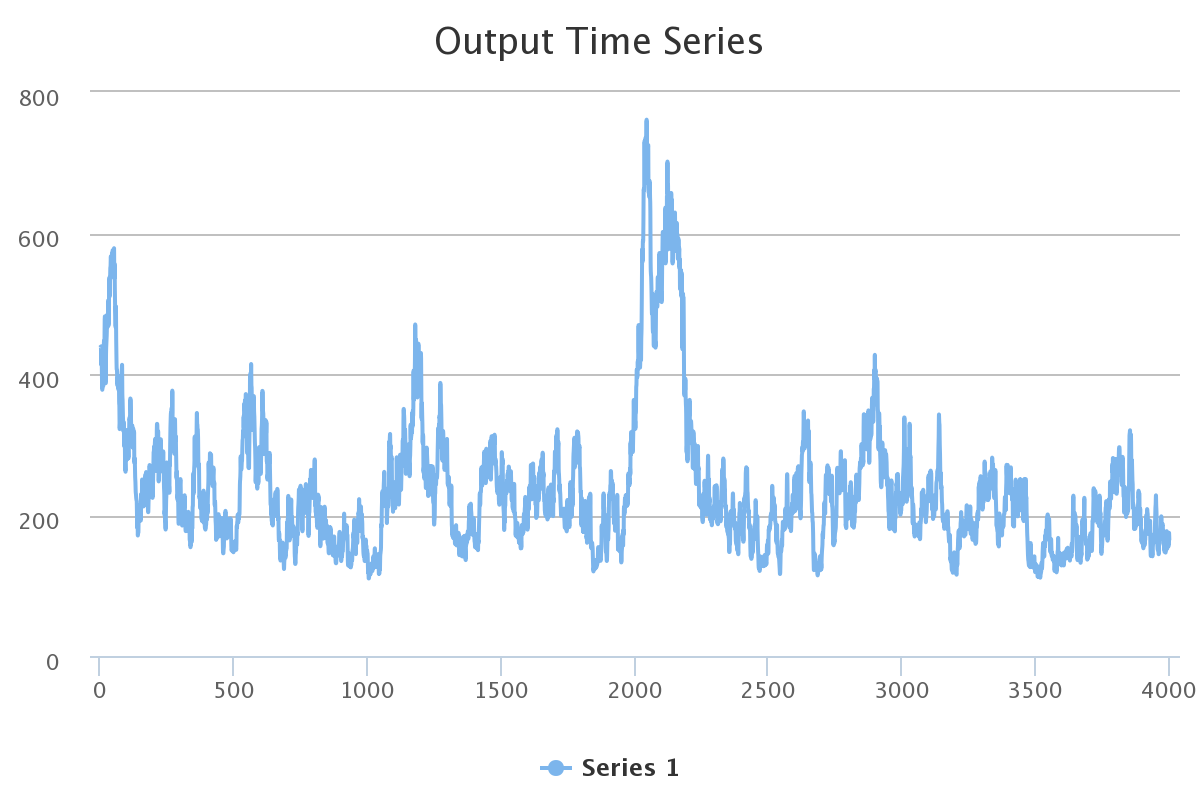
\includegraphics[width=0.75\textwidth]{timeseries-problem-iii.png}
        \caption{Generated Data}
        \label{fig:TimeSeries-iii}
      \end{figure}
\end{frame}

\begin{frame}{Time Lags}
    \begin{figure}[h]
        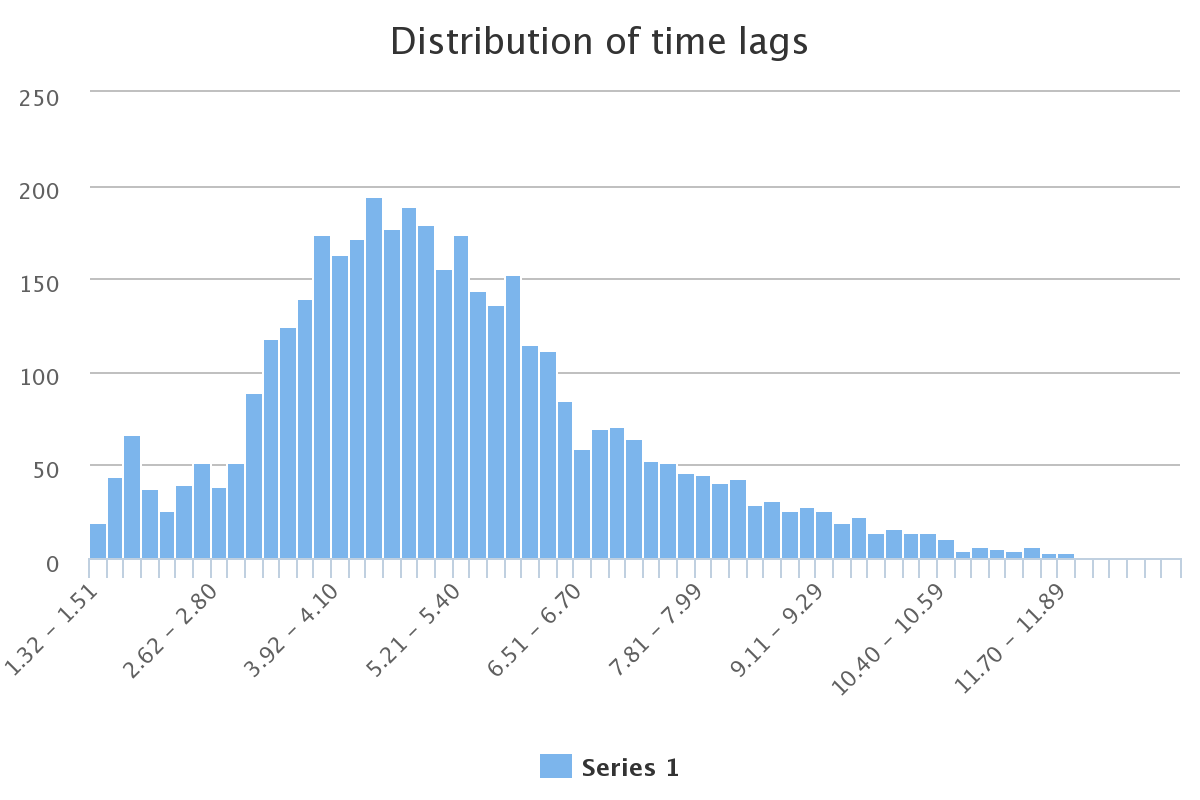
\includegraphics[width=0.75\textwidth]{data-hist-problem-iii.png}
        \caption{Time Lags}
        \label{fig:TimeLags-iii}
      \end{figure}
\end{frame}

\begin{frame}{Test Data Distribution}
    \begin{figure}[h]
        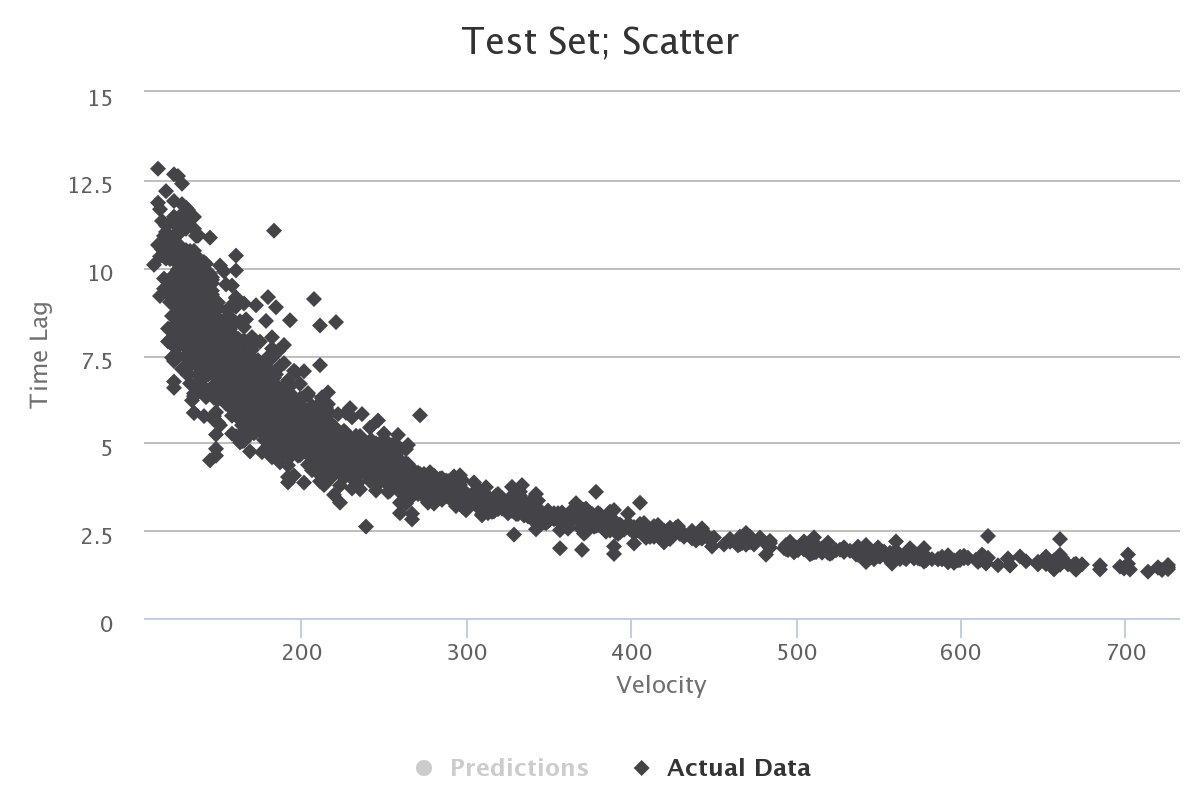
\includegraphics[width=0.75\textwidth]{data-scatter-iii.png}
        \caption{Output vs Time Lags}
        \label{fig:VelTimeLags-iii}
      \end{figure}
\end{frame}


\begin{frame}{Predictions}
    \begin{figure}[h]
        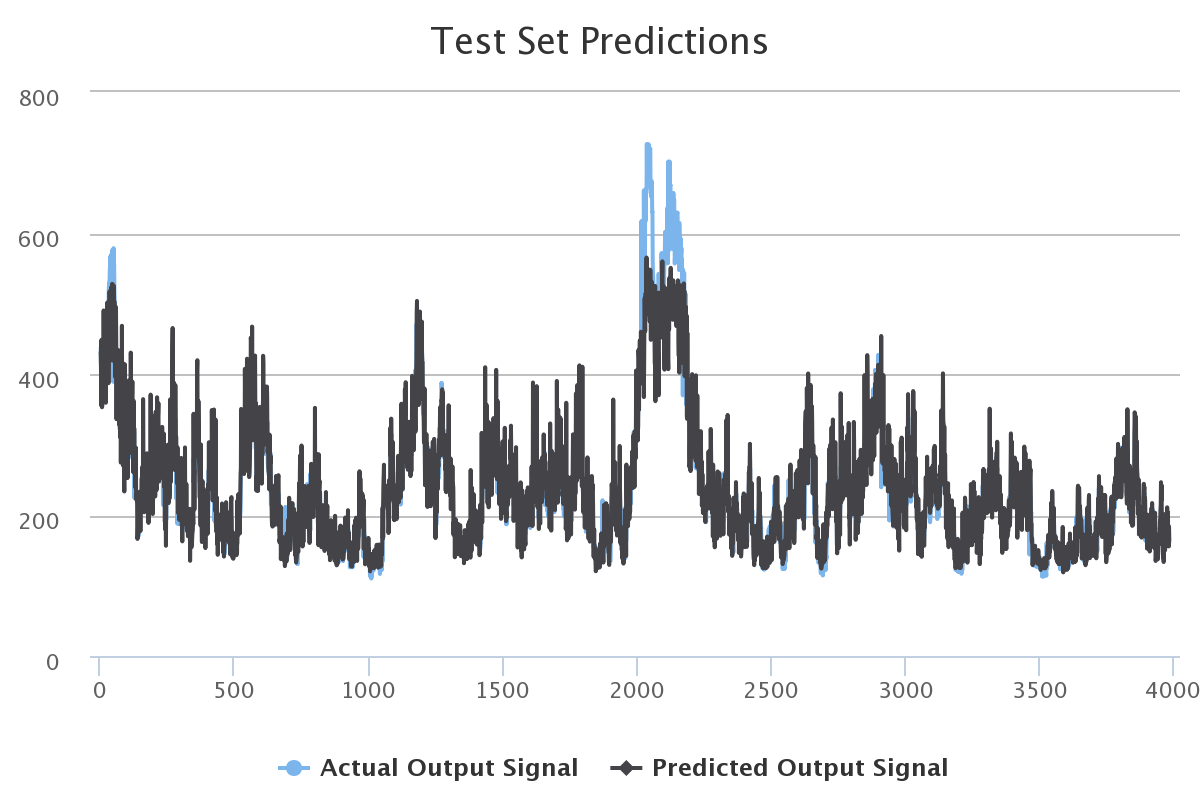
\includegraphics[width=0.75\textwidth]{predictions-iii.png}
        \caption{Test Set Time Series vs Predictions}
        \label{fig:predictions-iii}
      \end{figure}
\end{frame}

\begin{frame}{Errors}
    \begin{figure}[h]
        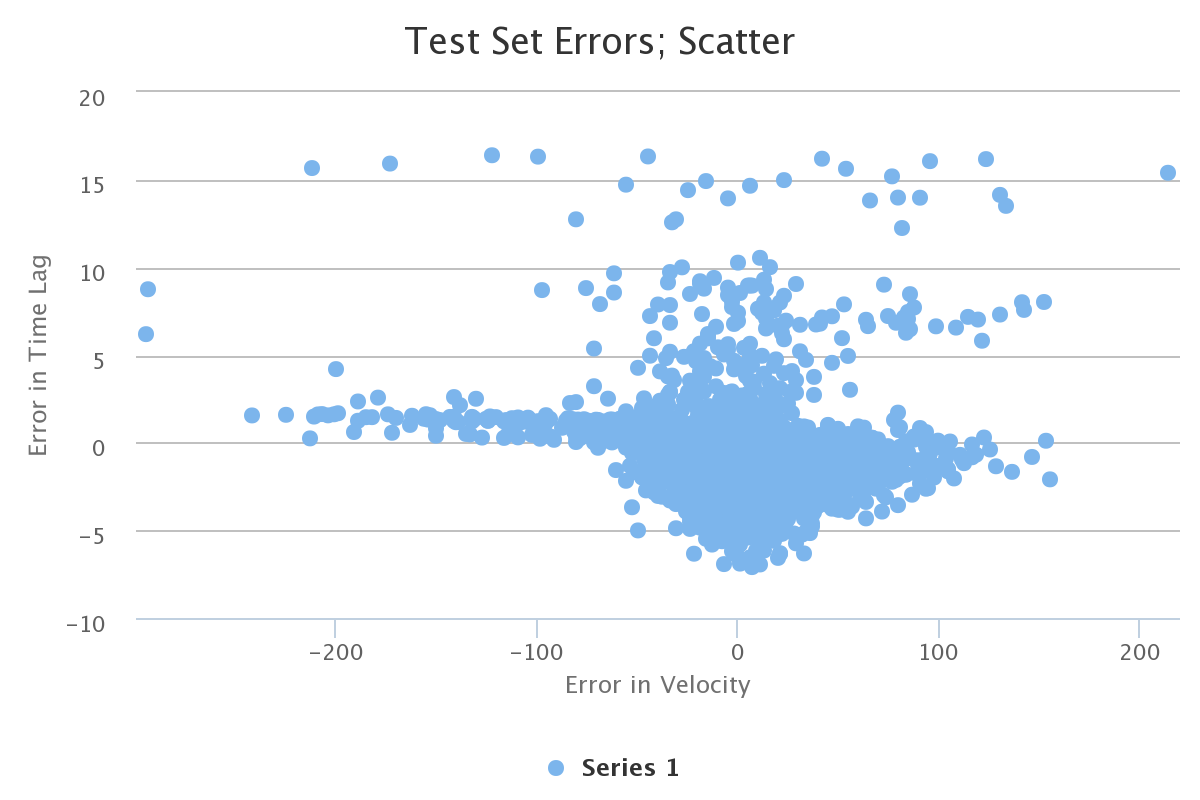
\includegraphics[width=0.75\textwidth]{errors-iii.png}
        \caption{Error in Output vs Error in Time Lag}
        \label{fig:errors-iii}
      \end{figure}
\end{frame}

\begin{frame}{Performance}
 
\begin{block}{Output}
\textbf{MAE}: 24.385 \\
\textbf{Pearson Corr}: 0.928 \\
\textbf{Spearman Corr}: 0.999
\end{block}

\begin{block}{Time Lag}
\textbf{MAE}: 1.758 \\
\textbf{Pearson Corr}: 0.415 \\
\textbf{Spearman Corr}: 0.999
\end{block}
\end{frame}


% All of the following is optional and typically not needed. 
\appendix
\section<presentation>*{\appendixname}
\subsection<presentation>*{For Further Reading}

\begin{frame}[allowframebreaks]
  \frametitle<presentation>{References}
        \bibliographystyle{apalike}
        \bibliography{references}
\end{frame}


\end{document}


